\documentclass[aspectratio=169,fontset=none]{ctexbeamer}
\setCJKmainfont{Microsoft YaHei}
\setCJKsansfont{Microsoft YaHei}
\setCJKmonofont{SimHei}
\usetheme{Madrid}
\usepackage{booktabs}
\usepackage{graphicx}

\title{一台虚拟机上的 LEBench}
\subtitle{SOSP 2019，Ren 等人}
\author{邹浩宇 \quad 5260000157}
\institute{CS340 操作系统}
\date{2026年11月9日}

\begin{document}

\begin{frame}
\titlepage
\end{frame}

\begin{frame}{论文声称什么}
\begin{itemize}
\item 从 Linux 3.0 到 4.20，核心内核操作变慢了（图 1）。
\item 例外是大块写和大块 munmap。
\item 十一个原因覆盖这些跳动：安全、新功能、错误配置（表 3、图 2）。
\item 关掉它们之后，Redis、Apache 和 Nginx 会变快（第 5 节）。
\end{itemize}
我们在作者的内核清单上检验第一条，并把一个安全开关当作扩展。应用程序只在一个内核上比较了 \texttt{spectre\_v2=off}。
\end{frame}

\begin{frame}{实际跑的是什么}
\begin{itemize}
\item 测量代码来自 LEBench 提交 \texttt{6aa7801}，没有改计时方法。
\item 同一条 K-best 规则：五个样本落在 5\% 以内，用 \texttt{clock\_gettime} 计时。
\item 循环缩短到 \texttt{BASE\_ITER} 40，这样每次启动可以重复三次。
\item Ubuntu 16.04.6 跑在 VirtualBox 里，传统 BIOS，磁盘在 \texttt{D:}。
\item 每个内核一次 \texttt{grub-reboot}。panic 后回到 4.4.0-210。
\end{itemize}
\end{frame}

\begin{frame}{为什么数字不是论文里的数字}
\begin{itemize}
\item 客户机：2 个 vCPU，4\,GB，虚拟磁盘，宿主机开了内存完整性。
\item CPU：i7-13700H。Meltdown：不受影响。
\item 论文的服务器是 Xeon E5-2630 v3，128\,GB。
\item 我们只在这台客户机上比较内核。不去对齐论文的纳秒数。
\end{itemize}
\end{frame}

\begin{frame}{扩展：只改一个开关 \texttt{nopti}}
同一内核（4.4.0-210），同一二进制，只改命令行。
\begin{itemize}
\item getpid：314\,ns 对 295\,ns。区间重叠。
\item 小块读、send、recv、select、poll、epoll 的区间也重叠。
\item fork：93\,$\mu$s 对 254\,$\mu$s。区间不重叠，方向和 KPTI 开销相反。
\item 两次启动的 \texttt{/sys/.../meltdown} 都是“Not affected”。
\end{itemize}
完整的表在报告里。
\end{frame}

\begin{frame}{\texttt{nopti} 说明了什么}
\begin{itemize}
\item 漏洞文件写明这颗 CPU 不受 Meltdown 影响。
\item getpid、读、send、recv 的变化小于各次运行之间的波动。
\item 加上 \texttt{nopti} 之后 fork 更慢，这不是论文里的 KPTI 故事。
\item KPTI 开销在这里没有复现出来。这颗 CPU 本来就不付这笔代价。
\end{itemize}
\end{frame}

\begin{frame}{扩展：批量计时 getpid}
只改一处：一次计时 1{,}000 次调用，再除以 1{,}000。K-best 和机器不变。
\begin{itemize}
\item 4.0.5：从 245 $\pm$ 0 ns 降到 129 $\pm$ 0 ns。区间不重叠。
\item 4.4.0-210：从 314 $\pm$ 39 ns 降到 127 $\pm$ 40 ns。
\item 批量之后这两个内核的区间重叠。单次计时里的变慢没有留下来。
\item 4.0.5 上一次空跑的时钟大约 130 ns。原来的 getpid 一行主要就是这一对时钟。
\end{itemize}
\end{frame}

\begin{frame}{各内核之间}
比 4.0.5 更晚的 19 个内核、627 项测量里，271 项（43\%）均值更高，76 项（12\%）至少高 50\%。117 项的区间不重叠且均值更高。

\IfFileExists{generated/relative_latency.pdf}{%
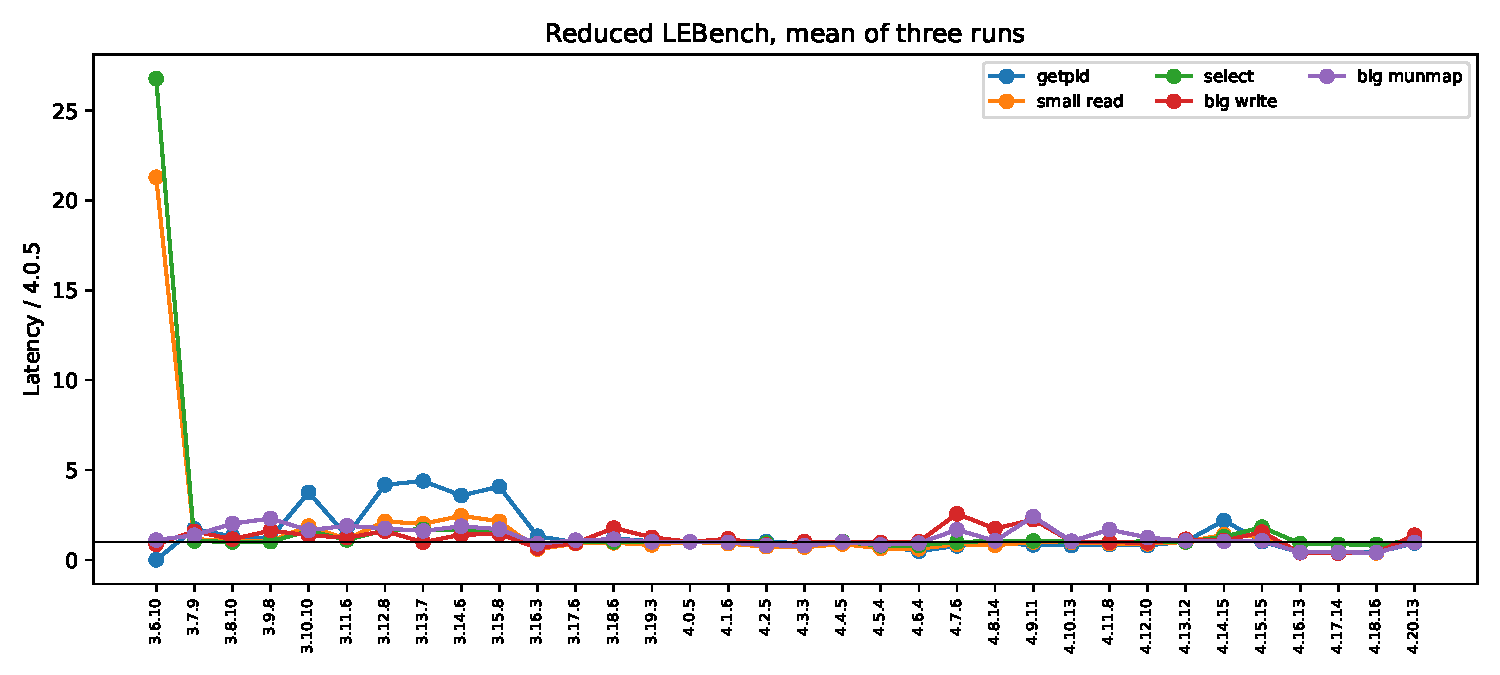
\includegraphics[width=\linewidth,height=0.52\textheight,keepaspectratio]{generated/relative_latency.pdf}
}{相对延迟图在 4.0.5 和更晚的内核都有三次运行之后才会写出。}
\end{frame}

\begin{frame}{一份没有采用的重写}
另一套 C 程序用 \texttt{rdtsc} 重写了测试，结果表是空的。
\begin{itemize}
\item 在这台虚拟机上，\texttt{rdtsc} 不是合适的时钟。
\item \texttt{select} 在计时区间里做了分配。
\item 上下文切换是一次平均值，不是 K-best，也没有把优先级调到 $-20$。
\item 它没有在 Linux 上执行过。
\end{itemize}
课程这棵树调用的是 \texttt{OS\_Eval}，没有把它换掉。
\end{frame}

\begin{frame}{论断 3：只改一个开关}
同一内核 4.4.0-210，各三次。Redis 4.0.8，Apache 2.4.18，Nginx 1.10.3。
\begin{itemize}
\item 漏洞文件从 Enhanced IBRS 变成 Vulnerable。
\item Apache 从每秒 1580 $\pm$ 139 次降到 1308 $\pm$ 24 次。更慢，区间不重叠。
\item Nginx 从每秒 5725 $\pm$ 966 次升到 7314 $\pm$ 208 次。更快，区间不重叠。
\item Redis 的均值上升，每个区间仍然重叠。
\item 论文的加速来自关掉全部十一项。这一个开关复现不出来。
\end{itemize}
\end{frame}

\begin{frame}{结论}
41 个列出的内核里，34 个完成了三次运行。3.0.7--3.5.4 的 sshd 没有应答。4.19.11 没有可下载的 modules 包。
\begin{itemize}
\item 论断 1：在这里不成立。更晚内核里 43\% 的均值高于本机 4.0.5，12\% 至少高 50\%。
\item 19 个更晚内核里，getpid 有 9 个明显更快，2 个更慢。
\item 论断 2：\texttt{nopti} 没有复现 KPTI 开销。这颗 CPU 不受影响。
\item 论断 3：不成立。\texttt{spectre\_v2=off} 让 Apache 变慢、Nginx 变快。Redis 仍落在波动里。
\item 总体：部分复现。缺的是论文自己的结论，测量框架已经跑起来了。
\end{itemize}
\end{frame}

\begin{frame}{两种安静的失败}
\begin{itemize}
\item 计时器选错时，抄来的基准程序仍然会打出一个数字。
\item 内核包装得上，却可能永远到不了 sshd。
\item 两种情况都要留在日志里：要么是一份 CSV，要么是一行启动失败。
\item 没有使用上游那个把 \texttt{grub-install} 装到分区上的做法。它可能写错磁盘。
\end{itemize}
\end{frame}

\end{document}
